\chapter{IMPLEMENTASI}
	Bab ini membahas implementasi sistem Pengendali Elastisitas secara rinci. Pembahasan dilakukan secara rinci untuk setiap komponen yang ada, yaitu: \textit{docker registry}, \textit{master host}, \textit{controller}, \textit{load balancer}, dan dasbor.
    
    \section{Lingkungan Implementasi}
    	Lingkungan implementasi dan pengembangan dilakukan menggunakan. Perangkat lunak yang digunakan dalam pengembangan adalah sebagai berikut:
        \begin{itemize}
        \item Sistem Operasi Linux Ubuntu Server 14.04 LTS
        \item Docker CE
        \item Python 2.7
        \item Redis
        \item MySQL
        \item Flask
        \item JMeter 3.2
        \end{itemize}
        
	\section{Implementasi Docker \textit{Registry}}
    	\textit{Docker registry} dibangun pada \textit{server} dengan IP \texttt{139.59.97.244} dan dapat diakses dari domain \texttt{https://registry.nota-no.life}. \textit{Docker registry} dapat digunakan setelah melakukan pemasangan \textit{server docker registry} seperti yang dijelaskan pada Lampiran \ref{install:dockerRegistry}.
        \subsection{Pengaturan \textit{Notification}}
        	Setelah melakukan pemasangan, selanjutnya adalah menambahkan konfigurasi untuk memberitahu \texttt{server controller} jika terjadi suatu kejadian pada \textit{docker registry}, seperti \textit{push} dan \textit{pull image}. Pada pengembangan sistem ini, kejadian yang diperlukan adalah \textit{push}, yaitu saat pengembang memasukkan aplikasi baru atau memperbarui aplikasi yang sudah ada di Docker \textit{registry}. Jika pengembang melakukan \textit{push} suatu aplikasi ke \textit{docker registry}, baik itu merupakan aplikasi pertama yang dimasukkan atau memperbarui aplikasi yang sudah ada, maka \textit{docker registry} akan memberitahukan kejadian tersebut kepada \texttt{server controller}. Untuk melakukan hal tersebut, buat folder \texttt{registry} di dalam folder \texttt{docker-registry}. Kemudian di dalamnya buat berkas dengan nama \texttt{config.yml} seperti Kode Sumber \ref{configregistry}.
    \begin{lstlisting}[frame=single,tabsize=2,breaklines,caption={Isi config.yml},label=configregistry, captionpos=b]
version: 0.1
log:
  fields:
    service: registry
storage:
  cache:
    blobdescriptor: inmemory
  filesystem:
    rootdirectory: /var/lib/registry
http:
  addr: :5000
  headers:
    X-Content-Type-Options: [nosniff]
health:
  storagedriver:
    enabled: true
    interval: 10s
    threshold: 3
notifications:
  endpoints:
    - name: alistener
      url: http://controller.nota-no.life/docker-registry-endpoint
      timeout: 60000ms
      threshold: 5
      backoff: 1s       
	\end{lstlisting}
            \indent Pada Kode Sumber \ref{configregistry} dapat dilihat bahwa \textit{notification} akan dikirimkan ke \textit{server host} melalui \textit{endpoint} \texttt{http://controller.nota-no.life/docker-registry-endpoint}. \textit{Timeout} yang digunakan adalah 60000 ms (\textit{milisecond}) atau 1 menit. \textit{Timeout} berguna jika \texttt{server controller} tidak memberikan balasan dalam waktu 1 menit, maka Docker \textit{registry} akan mencoba untuk mengirim ulang pemberitahuannya sampai dipastikan bahwa \texttt{server controller} sudah menerima pesannya dengan baik.
            
        \subsection{Melakukan Akses Terhadap \textit{Docker Registry}}
        	\textit{Docker registry} dapat diakses dari komputer yang memiliki mesin \textit{docker} di dalamnya. Sebelum dapat mengakses \textit{docker registry}, perlu menambahkan CA (\textit{Certification Authority}) dari Let's Encrypt pada komputer yang digunakan. Untuk melakukan proses tersebut buka folder \texttt{/usr/local/share/ca-certificates} dan buat berkas dengan nama \texttt{docker-regsitry.crt} di dalamnya. Masukkan Kode Sumber \ref{letsencryptpem} untuk mengisi berkasnya. Setelah itu simpan berkas dan perbarui CA dengan menjalankan \texttt{sudo update-ca-certificates}. Langkah terakhir adalah melakukan restart terhadap \textit{service docker} yang sedang berjalan dengna menggunakan perintah \texttt{sudo service docker restart}. Setelah proses di atas, selanjutnya adalah melakukan \textit{login} dengan menggunakan perintah \texttt{docker login https://registry.nota-no.life}. Masukkan \textit{username} dan \textit{password} yang sesuai, dan jika berhasil masuk akan muncul tulisan \texttt{Login Succeeded} yang menandakan sudah berhasil melakukan akses terhadap \textit{docker registry}.
            
        \subsection{Menambahkan dan memperbarui aplikasi}
        	Setelah berhasil terhubung dengan \textit{docker registry}, selanjutnya dapat mencoba untuk melakukan interaksi dengan menambahkan aplikasi baru ke dalamnya. Untuk melakukan percobaan, penulis melakukannya dengan perangkat lunak nginx dalam format \textit{docker} yang disediakan oleh Docker Hub. Untuk melakukan unduh, jalankan perintah berikut pada Kode Sumber \ref{pullnginx}. \\
\begin{lstlisting}[frame=single,tabsize=2,breaklines,caption={Perintah \textit{Pull} Nginx},label=pullnginx, captionpos=b]
docker pull nginx
\end{lstlisting}
            \indent Setelah berhasil diunduh, selanjutnya jalankan perangkat lunak nginx dengan menggunakan perintah yang tertera pada Kode sumber \ref{runnginx}. \\
\begin{lstlisting}[frame=single,tabsize=2,breaklines,caption={Perintah Menjalankan \textit{Image} Nginx},label=runnginx, captionpos=b]
docker run --name tesnginx nginx
\end{lstlisting}
            \indent Parameter \texttt{--name} berguna untuk memberikan nama pada \textit{container} agar mudah dikenali dimana lokasi aplikasi saat dijalankan. Pada kasus ini \textit{container} diberi nama dengan \texttt{tesnginx}. Setelah menjalankannya, \textit{container} yang terbentuk dapat digunakan lebih lanjut, misalnya dengan mengubah data yang ada didalamnya, menambahkan fitur baru, atau hanya sekedar mengganti nama dari aplikasi. Setelah melakukan modifikasi terhadap \textit{container}, jika ingin membuat \textit{images} baru dari \textit{container} tersebut, maka hal pertama yang harus dilakukan adalah menghentikan \textit{container} yang sedang berjalan dengan menggunakan perintah \texttt{docker stop tesnginx} untuk kasus yang digunakan oleh penulis. Setelah itu lakukan \textit{commit} dengan menjalankan perintah seperti pada Kode Sumber \ref{commitnginx}.
\begin{lstlisting}[frame=single,tabsize=2,breaklines,caption={Perintah \textit{Commit Container} Nginx},label=commitnginx, captionpos=b]
docker commit tesnginx registry.nota-no.life/ tesnginx:1.0
\end{lstlisting}
            \indent Parameter keempat pada perintah di atas adalah \texttt{registry.nota-no.life/tesnginx:1.0} yang merupakan penamaan \textit{image} yang terbentuk. Parameter tersebut memiliki tiga bagian dengan pola seperti \texttt{[URL]/[nama]:[versi]}. Artinya membuat \textit{image} dengan URL \textit{repository} ada pada \texttt{registry.nota-no.life}. Kemudian nama dari \textit{image}-nya sendiri adalah \texttt{tesnginx} dan versinya adalah \texttt{1.0}. Setelah melakukan commit, maka \textit{image} baru akan terbentuk. Langkah terakhir adalah melakukan \textit{push image} ke \textit{docker registry} yang tersedia dengan menggunakan perintah seperti Kode Sumber \ref{pushnginx}. \\
\begin{lstlisting}[frame=single,tabsize=2,breaklines,caption={Perintah \textit{Push Image} Terbaru Nginx},label=pushnginx, captionpos=b]
docker push registry.nota-no.life/tesnginx:1.0
\end{lstlisting}
            \indent Untuk memperbarui aplikasi yang sudah diungguh pada \textit{docker registry}, proses yang dilakukan sama dengan menambahkan aplikasi baru.
    
    \section{Implementasi Master Host}
    	Master Host merupakan \textit{server} yang digunakan untuk menjalankan semua \textit{container} dari aplikasi. \textit{Server} ini memiliki IP publik, yaitu \texttt{128.199.182.29}. \textit{Server} ini menyediakan sebuah \textit{endpoint} dengan port 5000 yang digunakan oleh \textit{server} pengendali untuk melakukan komunikasi. \textit{Endpoint} dibangun dengan menggunakan perangkat kerja Flask. Lalu, interaksi dengan \textit{docker deamon} menggunakan pustaka docker-py. Penggunaan pustaka tersebut agar interaksi dapat dilakukan dengan mudah. \\
        \indent Berikut adalah penjelasan \textit{endpoint} yang disediakan oleh \textit{server} ini:
        \begin{itemize}
        \item \texttt{/start\_container} \\
        	Rute ini memiliki metode \texttt{POST} dan berguna untuk menjalankan atau memulai suatu \textit{container} dari suatu aplikasi. \textit{Endpoint} ini akan dipanggil oleh \textit{server} Controller jika ada permintaan dari pengguna untuk menjalankan aplikasi dan membuat \textit{container} baru untuk memenuhi kebutuhan aplikasi. Saat akan membuat \textit{container} baru, akan dilakukan pengecekan apakah \textit{image} dari aplikasi yang akan dijalankan sudah ada atau belum. Jika \textit{image} tidak ada, maka terlebih dahulu akan melakukan \textit{pull} dari \textit{server} \textit{docker registry}. \\
        \item \texttt{/delete\_container/<container\_id>} \\
        	Rute ini memiliki metode \texttt{GET} dan berguna untuk menghentikan aplikasi dan menghapus satu \textit{container} dari aplikasi yang sedang berjalan. Rute ini digunakan saat pengguna ingin menghentikan aplikasinya atau aplikasi kelebihan jumlah \textit{container}, sehingga harus mengurangi \textit{container} yang sedang berjalan. Untuk menghapus container yang sedang berjalan, maka \textit{container} pertama kali harus dihentikan prosesnya, kemudian menghapusnya. \\
        \item \texttt{/container\_info} \\
        	Rute ini digunakan untuk mendapatkan data dari satu atau lebih \textit{container}. Data yang akan dihasilkan yaitu penggunaan\textit{ memory} dan CPU dari \textit{container} yang sedang berjalan. \\
        \end{itemize}
    
    \section{Implementasi Server Controller}
    	\textit{Server} \textit{controller} merupakan \textit{server} yang akan mengelola keseluruhan data dari sistem. Pada \textit{server} ini semua keputusan yang dilakukan oleh sistem dilakukan, seperti menambahkan dan menghapus \textit{container}, menjalankan, memperbarui, dan menghapus aplikasi, dan memperbarui konfigurasi \textit{load balancer}. \textit{Server controller} memilik IP 128.199.250.137 dan domain \textit{http://controller.nota-no.life} yang digunakan oleh dasbor. Selain itu, \textit{server} dapat diakses melalui port 5000.
    	\subsection{\textit{Endpoint Docker Regsitry}}
        	\textit{Server docker registry} akan mengirimkan suatu kejadian jika terjadi perubahan pada datanya. Oleh karena itu, \textit{server} Controller memiliki rute \texttt{/docker-registry-endpoint} dengan metode \texttt{POST} yang akan menangkap pesannya.\\
            \indent Data yang diterima berupa data dalam format JSON. Data yang akan diproses semuanya berada di dalam \textit{key} \texttt{events}. Di dalam data \texttt{events}, selanjutnya \textit{key} yang akan digunakan adalah \textit{key} \texttt{action} dan \texttt{target}. \\
            \indent \textit{Key} \texttt{action} akan memberitahu kejadian apa yang sedang terjadi. Umumnya isi yang sering muncul adalah \textit{string} \texttt{push} dan \texttt{pull}. \textit{string} \texttt{push} menunjukkan adanya kejadian saat pengembang memasukkan aplikasi baru atau memperbarui aplikasi yang sudah ada di \textit{docker registry}. Lalu \textit{string} \texttt{pull} adalah nilai yang menunjukkan kejadian saat ada suatu host yang mengambil sebuah \textit{image} dari \textit{docker registry}. Dalam pengembangan sistem ini, proses hanya akan dilanjutkan jika bernilai \texttt{push} yaitu saat ada yang melakukan perubahan data \textit{image} pada \textit{docker registry} dan mengabaikan jika ada \textit{host} yang melakukan unduh \textit{image}.\\
            \indent \textit{Key} \texttt{target} memiliki beberapa data di dalamnya, dan \textit{key} yang digunakan adalah \texttt{host}, \texttt{repository}, \texttt{tag}, dan  \texttt{mediatype}. \textit{Key} \texttt{host} menunjukkan letak alamat, dalam bentuk URL atau IP, dari \textit{docker registry}. \textit{Key} \texttt{repository} merupakan nama dari \textit{image} atau aplikasi yang ada di dalam \textit{event}. \textit{Key} \texttt{tag} menunjukkan versi atau jenis dari \textit{image}. Misalnya bernilai \texttt{1.0}, maka menunjukkan bahwa \textit{image} tersebut berada dalam versi 1.0. Lalu ada juga \texttt{tag} yang berisi nilai \texttt{demo}, berarti kemungkinannya \textit{image} tersebut untuk keperluan percobaan.\\
            \indent Lalu terakhir ada \textit{key} \texttt{mediatype}. Dalam  mengirimkan \textit{notification}, \textit{docker registry} tidak hanya melakukannya sekali dalam satu \textit{event}, tapi bisa saja beberapa kali, sesuai dengan \textit{event} yang terjadi. Misal \textit{event} \texttt{push}, bisa saja untuk melakukan \textit{event} tersebut diperlukan lebih dari satu proses  Untuk menanganinya. Masing-masing proses tersebutlah yang akan dikirimkan. Agar tidak terjadi tabrakan pemroses \textit{event} yang sama, diperlukan pengecekan \texttt{mediatype}. Proses hanya akan dilanjutkan jika \textit{key} tersebut bernilai \texttt{application/vnd. docker.distribution.manifest.v2+json}. \\
            \indent Selanjutnya adalah pengecekan apakah \textit{image} sudah ada di dalam basis data. Jika data \textit{image} belum ada, maka data yang baru tersebut akan dimasukkan ke dalam basis data. Proses akan berakhir sampai disana jika itu merupakan \textit{image} baru. Untuk menjalankan aplikasinya bisa melalui dasbor. Lalu jika \textit{image} yang diproses sudah ada ada di dalam basis data, maka masukkan data baru ke dalam basis data. Biasanya penambahan data baru ini yang berbeda hanya data \texttt{tag}-nya saja. Selanjutnya adalah mengecek apakah \textit{image} tersebut sedang berjalan atau dengan kata lain ada \textit{container} yang sedang aktif menggunakan \textit{image} itu. Jika ada maka buat \textit{container} dari \textit{image} yang baru sejumlah \textit{container} dari image lama. Setelah \textit{container} semua \textit{container} baru terbentuk, baru hapus \textit{container} dari \textit{image} lama dan perbarui pengaturan \textit{load balancer}. \\
            \indent Semua pemrosesan data yang dikirim oleh \textit{docker registry} dilakukan dengan memasukkannya ke dalam Redis. Kemudian ada \textit{worker} yang akan membaca data yang masuk ke Redis dan menjalankan fungsinya sehingga pemrosesan di atas akan dilakukan secara \textit{asynchronous}.Hal tersebut dilakukan agar \textit{docker registry} bisa mendapatkan balasan secepat mungkin dari \textit{server} Controller. Jika tidak dimasukkan ke dalam Redis, maka pemrosesan yang dilakukan di atas harus diselesaikan terlebih dahulu sebelum bisa memberikan balasan.
            
        \subsection{Skema Basis Data Controller Menggunakan MySQL}
        	Untuk mengelola data yang ada pada sistem, dibutuhkan basis data sebagai tempat penyimpanannya, yaitu MySQL. MySQL \textit{server} yang digunakan adalah versi 5.5.55. Data yang disimpan antara lain adalah data dari \textit{image} yang ada di \textit{docker registry}, data \textit{container} yang sedang berjalan pada \textit{server master}, dan data domain untuk masing-masing \textit{image} atau aplikasi.
            MySQL \textit{server} memiliki definisi tabel \texttt{images}, \texttt{containers}, dan \texttt{domains}. Table \texttt{images} digunakan untuk menyimpan data \textit{image} yang ada di \textit{server} \textit{docker registry}. Berikut definisi tabel \texttt{images} pada Table \ref{tabelImages}.
        
        \begin{longtable}{|p{0.03\textwidth}|p{0.20\textwidth}|p{0.20\textwidth}|p{0.41\textwidth}|}
			\caption{Tabel images} \label{tabelImages} \\
			\hline
			\textbf{No} & \textbf{Kolom} & \textbf{Tipe} & \textbf{Keterangan} \\ \hline
			\endhead
			\endfoot
			\endlastfoot
			1 & id & int & Sebagai primary key pada tabel, nilai awal adalah \texttt{AUTO\_INCREMENT}. \\ \hline
			2 & host & varchar(50) & Menunjukkan URL atau IP dari \textit{docker registry} untuk mengunduh \textit{image}. \\ \hline
			3 & repository & varchar(50) & Nama aplikasi. \\ \hline
			4 & tag & varchar(50) & Versi atau label yang diberikan kepada sebuah \textit{image}. \\ \hline
			5 & domain & varchar(50) & Domain yang diberikan oleh sistem untuk \textit{image} yang bersangkutan. \\ \hline
			6 & port & int & Port dari \textit{image} yang dibuka untuk \textit{host} saat dijalankan. \\ \hline
			7 & version & int & Penomoran urutan \textit{image} yang masuk ke dalam sistem. \\ \hline
            8 & isRunning & int & Status apakah image sedang berjalan (1), proses untuk dijalankan atau dimatikan (2), dan juga mati (0). \\ \hline
		\end{longtable}
        
        \indent Tabel \texttt{containers} digunakan untuk menyimpan data \textit{containers} yang sedang berjalan pada \textit{server master host}. Penyimpanan ini diperlukan agar mempercepat dan mempermudah saat mengolah data \textit{container} karena tidak perlu memintanya secara langsung dari \textit{server master}. Definisi tabel \texttt{containers} seperti pada Tabel \ref{tabelContainers}.
        
        \begin{longtable}{|p{0.03\textwidth}|p{0.20\textwidth}|p{0.20\textwidth}|p{0.41\textwidth}|}
			\caption{Tabel containers} \label{tabelContainers} \\
			\hline
			\textbf{No} & \textbf{Kolom} & \textbf{Tipe} & \textbf{Keterangan} \\ \hline
			\endhead
			\endfoot
			\endlastfoot
			1 & id & int & Sebagai primary key pada tabel, nilai awal adalah \texttt{AUTO\_INCREMENT}. \\ \hline
			2 & image\_id & int & \textit{Foreign key dari} \textit{image} yang merujuk ke table images. \\ \hline
			3 & container\_id & varchar(50) & ID dari containers yang sedang berjalan. ID didapatakan dari \textit{server master} saat pembuatan \textit{container} berhasil dilakukan.  \\ \hline
			4 & port & int & Merupakan \textit{port} dari \textit{container} yang diberikan oleh \textit{host}. \\ \hline
			5 & status & varchar(50) & Status apakah \textit{container} dalam keadaan sedang berjalan atau mati. \\ \hline
		\end{longtable}
        
        \indent Tabel \texttt{domains} digunakan untuk menyimpan ID record dari domain yang didaftarkan ke DNS DigitalOcean. ID record digunakan untuk menghapus domain yang terdaftar jika sudah tidak dibutuhkan lagi. Definisi tabel \texttt{domains} seperti pada Tabel \ref{tabelDomains}
        
        \begin{longtable}{|p{0.03\textwidth}|p{0.20\textwidth}|p{0.20\textwidth}|p{0.41\textwidth}|}
			\caption{Tabel domains} \label{tabelDomains} \\
			\hline
			\textbf{No} & \textbf{Kolom} & \textbf{Tipe} & \textbf{Keterangan} \\ \hline
			\endhead
			\endfoot
			\endlastfoot
			1 & id & int & Sebagai primary key pada tabel, nilai awal adalah \texttt{AUTO\_INCREMENT}. \\ \hline
			2 & domain & varchar(50) & Menyimpan subdomain. \\ \hline
			3 & record\_id & varchar(50) & ID dari domain yang diberikan oleh DigitalOcean saat memasukkan domain baru. \\ \hline
		\end{longtable}
 
 		\subsection{Menambahkan dan Menghapus Domain}
        	\begin{figure}[H]
				\centering
				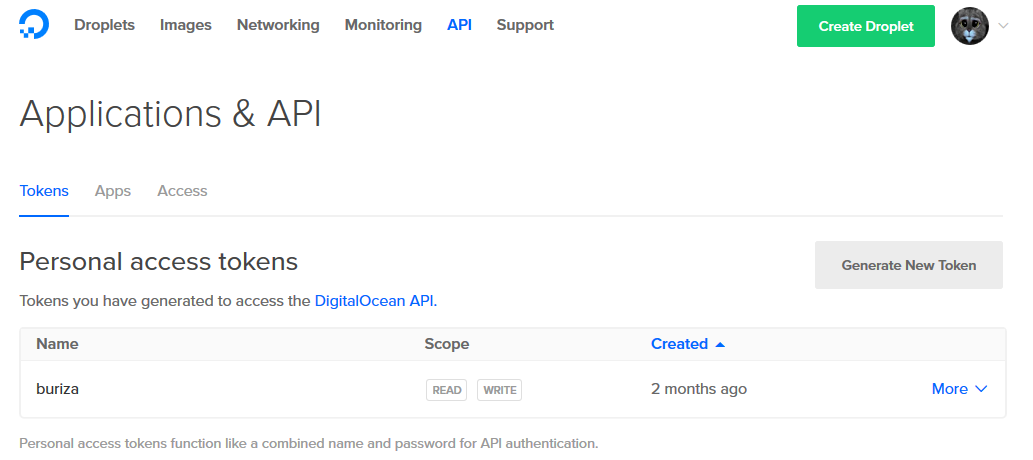
\includegraphics[width=10cm,height=5cm]{Images/C-4/docp.png}
				\caption{DigitalOcean Control Panel}
				\label{docp}
			\end{figure}
        	Domain yang digunakan dikelola oleh DigitalOcean. Untuk melakukan interaksi, seperti menambahkan record domain baru, pada pengembangan Tugas Akhir ini menggunakan API dalam bahasa pemrograman \texttt{curl} yang disediakan.
            \indent Hal pertama yang harus dilakukan adalah mendapatkan token untuk dapat mengakses API. Token bisa didapatkan dari \textit{control panel} Digital Ocean, seperti pada Gambar \ref{docp}.
        
        	\indent Setelah mendapatkan token, langkah selanjutnya adalah melakukan akses menggunakan \texttt{Curl} API. Namun, dalam implementasi pada Tugas Akhir ini, \texttt{curl} diganti dengan pustaka \texttt{requests} pada Python dan metode yang digunakan adalah \texttt{POST}.\\
            \indent Dalam melakukan permintaan ke API, hal pertama yang perlu disiapkah adalah \texttt{header}. Pada bagian ini, diperlukan dua \textit{key}. Yang pertama yaitu \texttt{Content-Type} yang berisi nilai \texttt{application/json}. Lalu yang kedua adalah \texttt{Authorization} dengan nilai sesuai dengan token yang didapatkan sebelumnya.\\
            \indent Untuk datanya sendiri diperlukan tiga \textit{key}, yaitu \texttt{type}, \texttt{name}, dan \texttt{data}. Untuk key \texttt{type} digunakan untuk menentukan jenis \textit{record} DNS dan nilai yang digunakan adalah \texttt{A}. Nilai \texttt{A} menunjukkan suatu domain atau subdomain, dalam kasus ini subdomain, ke suatu IP. Selanjutnya \textit{key} \texttt{name} digunakan untuk menentukan nama subdomain yang didaftarkan. Yang terakhir adalah \textit{key} \texttt{data}, menunjukkan IP yang adakn ditunjuk oleh domain yang didaftarkan. Untuk nilainya sendiri menunjuk IP \textit{server master}, yaitu \texttt{128.199.160.188}. Setelah semua siap, permintaan ke API bisa dilakukan. melalui URL \texttt{https://api.digitalocean.com/v2/domains/ <namaDomain>/records} Jika berhasil, maka akan mengembalikan status \texttt{201 Created} dan  ID dari \textit{record} yang didaftarkan.\\
            \indent Setelah suatu \textit{record} terdaftar, ada saatnya untuk menghapusnya jika tidak ada aplikasi yang menggunakannya. Untuk melakukan proses tersebut, metode yang digunakan adalah \texttt{DELETE}. Untuk \texttt{header} sama seperti menambahkan \textit{record}. Pada proses penghapusan \textit{record} tidak ada data yang dikirim. Permintaan dilakukan melalu URL \texttt{https://api.digitalocean.com/v2/domains/ <namaDomain>/records/<id\_record>}. Jika berhasil akan mengembalikan status \texttt{204 No Content}.

        \subsection{Implementasi Task Queue Menggunakan Redis}
        	Pada \textit{server} ini, banyak proses yang terjadi terdiri dari banyak subprosess lainnya. Proses yang terjadi semuanya berasal dari Flask yang merupakan sebuah perangkat kerja Web yang mana permintaan terhadap layanan melalui protokol HTTP. Jika proses yang panjang dibiarkan saja berjalan tanpa ada kendali lebih lanjut, maka balasan yang akan diberikan kepada klien yang meminta layanan akan menunggu seluruh proses berakhir. Bisa saja saat menjalankan proses tersebut terdapat kesalahan atau hubungan antara klien dan \textit{server} terputus yang menyebabkan proses berhenti ditengah jalan. Untuk mengatasi permasalah tersebut, digunakan prinsip \textit{task queue} menggunakan Redis. Jadi suatu proses akan dilemparkan ke dalam Redis, dan program akan 'melupakan' proses yang sudah diberikan kepada Redis sehingga melanjutkan menjalankan perintah yang diberikan, tidak peduli proses sebelumnya sudah dieksekusi atau belum. Setelah masuk ke dalam Redis, terdapat \textit{worker} yang akan menjalankan proses tersebut. Dengan cara tersebut, proses yang panjang akan bekerja dibelakang dan balasan atau koneksi antara klien dan \textit{server} tidak berlangsung lama, yang mengurangi kemungkinan terjadi kesalahan didalamnya.\\
            \indent Untuk melakukan hal tesebut, Redis harus terpasang, seperti yang dijelaskan pada \ref{install:redis}. Untuk terhubung dengan Redis, menggunakan pustaka RQ dan Redis untuk Pyhton seperti yang dijelaskan pada \ref{install:pythonlibrary}. Redis yang sudah terpasang secara umum akan berjalan pada port \texttt{6379}. Selanjutnya adalah membuat koneksi ke Redis dan menyiapkan \textit{queue} untuk menampung proses yang diberikan. Implementasinya seperti yang ditunjukkan pada Kode Sumber \ref{conRedis}  
        \begin{lstlisting}[frame=single,tabsize=2,breaklines,caption={Koneksi Redis},label=conRedis, captionpos=b]
con = redis.Redis('localhost', port=6379, db=0)
q = Queue(connection=con)
		\end{lstlisting}
        
        \subsection{Penyimpanan Konfigurasi Load Balancer pada etcd}
        	File konfigurasi HAProxy pada \textit{server load balancer} akan berubah secara otomatis karena confd yang berjalan akan membaca perubahan data pada etcd yang ada di \textit{server controller}. etcd sendiri berjalan pada port \texttt{5050}. Pada \textit{server controller} ini, disimpan data \textit{image}, \textit{container}, dan \textit{domain} dari aplikasi yang sedang berjalan. Penyimpanan data dilakukan dalam bentuk JSON. Untuk satu aplikasi, format yang digunakan seperti pada Kode Sumber \ref{etcd1}.
	\begin{lstlisting}[frame=single,tabsize=2,breaklines,caption={Format Penyimpanan Data \textit{Image} pada etcd},label=etcd1, captionpos=b]
{
	"image_name": image_name,
	"domain": domain,
	"containers": listContainers
}
	\end{lstlisting}
    
	\indent Lalu, sebuah data di dalam \textit{key} \texttt{containers} memiliki format seperti Kode Sumber \ref{etcd2}. Satu data menyatakan satu \textit{container} yang sedang berjalan. Jika ada pada suatu waktu ada tiga \textit{container} yang berjalan, maka data pada \textit{key} \texttt{containers} ada tiga buah.
    
    \begin{lstlisting}[frame=single,tabsize=2,breaklines,caption={Format Penyimpanan Data \textit{Container} pada etcd},label=etcd2, captionpos=b]
{
	"name": name,
	"ip": ip,
	"port": port
}    
	\end{lstlisting}
    
    \indent Untuk menyimpan dan menghapus data menggunakan pustaka \texttt{python-etcd}. Sedangkan untuk memastikan apakah data sudah masuk, bisa menggunakan \texttt{curl}. Perintah yang digunakan untuk menampilkan data adalah \texttt{curl http://localhost:5050/v2/keys/images/}.
    
    	\subsection{Implementasi Program Monitoring HAProxy}
        	Pada \textit{server controller} ini, \textit{log} yang dihasilkan dari HAProxy akan diproses. Data \textit{log} yang dihasilkan berupa data dalam format CSV. \textit{Server load balancer} akan mengirimkan semua data \textit{log} tersebut, tapi data yang diolah selanjutnya hanya menggunakan tiga kolom saja, yaitu pada indeks ke 0, 1, dan 7. Berikut adalah penjelasan untuk masing-masing kolom yang digunakan:
            \begin{enumerate}
            \item 0 \texttt{pxname} \\
            	Kolom \texttt{pxname} atau \textit{proxy name} menunjukkan nama aplikasi yang sedang berjalan. Dengan kata lain, kolom ini menunjukkan nama aplikasi atau \textit{image} yang ada di \textit{server master}.
            \item 1 \texttt{svname} \\
            	Kolom \texttt{svname} atau \textit{service name} menunjukkan \textit{container} yang dituju atau digunakan oleh suatu aplikasi. Permintaan pengguna ke suatu aplikasi akan diarahkan ke \textit{container} menggunakan data ini.
     		\item 7 \texttt{stot} \\
            	Kolom \texttt{stot} menunjukkan penggunakan akses ke service tersebut. Nilainya merupakan kumulatif semua \textit{request} yang diterima. Jika konfigurasi dari HAProxy diubah, maka nilainya akan kembali ke nol.
            \end{enumerate}
                      \indent Hasil data yang didapatkan di atas akan dimodelkan menggunakan ARIMA untuk mendapatkan prediksi \textit{request} ke depannya. Untuk model ARIMA sendiri dibangun berdasarkan \textit{dataset log request} ke website World Cup 1998 selama 92 hari \cite{noauthor_1998_nodate}. Data yang di dapatkan pertama kali diolah dari dari data biner ke dalam format csv. Setelah itu mengecilkan data dengan mengelompokkannya untuk jarak waktu 1 jam untuk proses pembuatan model. Data \textit{request} kemudian dikecilkan dengan rasio mengambil 1000 \textit{request} asli untuk dijadikan 1 \textit{request} untuk model. 
            
            \subsection{Implementasi Program Monitoring Server Master}
            	Monitoring pada \textit{server} Master Host bertujuan untuk mengetahui jumlah penggunaan sumber daya CPU dan \textit{memory} dari \textit{container} yang sedang berjalan. Data status \textit{container} yang akan diberikan oleh Master Host merupakan data mentah dalam format JSON. Pada subsistem ini data tersebut akan diolah untuk mengetahui secara pasti berapa penggunaan CPU dan \textit{memory}. Hasil pengolahan data tersebut digunakan untuk perhitungan pada \textit{Reactive Model}. \\
                \indent Data penggunaan CPU didapatkan dengan melakukan perhitungan penggunaan CPU dalam selang waktu tertentu. Variable yang dibutuhkan untuk melakukan perhitungan didapatkan dari \textit{server} Master Host. Setelah mendapatkan data dalam format JSON, selanjutnya adalah menghitungnya menggunakan pseudocode yang tertera pada Kode Sumber \ref{calcpupercentage}.\\
                \begin{lstlisting}[frame=single,tabsize=2,breaklines,caption={Pseudocode Menghitung Penggunaan CPU},label=calcpupercentage, captionpos=b]
function calCPUPercent:
    cpuPercent <- 0.0
    cpuDelta <- float64(v.CPUStats.CPUUsage.TotalUsage) - float64(previousCPU)
    systemDelta <- float64(v.CPUStats.SystemUsage) - float64(previousSystem)
    if systemDelta > 0.0 AND cpuDelta > 0.0 
        cpuPercent = (cpuDelta / systemDelta) * float64(len(v.CPUStats.CPUUsage.PercpuUsage)) * 100.0
    return cpuPercent
			\end{lstlisting}
                \indent Untuk mendapatkan penggunaan \textit{memory} dari sebuah \textit{container}, dapat menggunakan \textit{key} dengan nama \textit{memory\_stats}. Nilai yang diberikan berupa penggunaan \textit{memory} dalam satuan \textit{byte}. Penggunaan satu buah \textit{container} dibatasi sampai 512 MB. Lalu batas atas dari penggunaannya adalah 80 \%. Jika ada \textit{container} yang melebihi batas atas tersebut, maka akan ditambahkan sebagai bagian dari \textit{container} yang melebihi batas penggunaan.
                \indent Setelah mendapatkan jumlah container yang melebihi batas penggunaan CPU dan memory, selanjutnya adalah menentukan jumlah container yang harus dibentuk menggunakan Reactive Model. Perhitungannya menggunakan rumus seperti yang tertera pada Kode Sumber \ref{calreactivemodel}. Variable \texttt{totalExceed} menunjukkan jumlah \textit{container} yang sudah melebihi batas penggunaan. Lalu variable \texttt{THRESHOLD\_RESOURCE} merupakan batas atas dari penggunaan sumber daya yang bernilai 0.8.
            \begin{lstlisting}[frame=single,tabsize=2,breaklines,caption={Perhitungan \textit{Reactive Model}},label=calreactivemodel, captionpos=b]
NReactive = math.ceil(totalExceed * (1 - THRESHOLD_RESOURCE) / THRESHOLD_RESOURCE)
			\end{lstlisting}
            
        \subsection{Implementasi Pengendali Elastasitas}
            Dengan menggunakan data yang dihasilkan dari sistem yang melakukan monitoring terhadap \textit{server} \textit{Load Balancer} dan Master Host, maka pada sistem ini hasil perhitungan dari kedua \textit{server} tersebut akan diputuskan. Pada perhitungan ini, di tentukan bahwa jumlah maksimal permintaan yang bisa diterima oleh satu \textit{container} adalah 500 buah, yang dinyatakan dengan variable $f$. \\
            \indent Dari perhitungan fungsi di atas, bisa diketahui berapa jumlah \textit{container} yang diperlukan aplikasi. Jika jumlah \textit{container} yang dibutuhkan lebih banyak dari jumlah \textit{container} yang sedang berjalan, maka \textit{container} baru akan dibuat. Namun jika jumlah \textit{container} yang sedang berjalan lebih banyak dari yang dibutuhkan, maka \textit{container} akan dikurangi. Ada perbedaan yang terjadi saat menambahkan dan mengurangi \textit{container}. Pada fungsi di atas, terdapat variable \texttt{DELAY\_SCALE\_IN}, yaitu pengurangan \textit{container} hanya akan terjadi jika pengecekan sudah diakukan sebanyak nilai tersebut. Jadi, pada kasus ini, pengurangan \textit{container} akan terjadi jika sudah terjadi pengecekan sebanyak 10 kali yang masing-masingnya konsisten bahwa jumlah \textit{container} yang berjalan lebih banyak dari yang diperlukan. Namun, jika diperlukan penambahan \textit{container}, maka akan dilakukan saat itu juga tanpa ada \textit{delay}.
            \begin{lstlisting}[frame=single,tabsize=2,breaklines,caption={Perhitungan \textit{Reactive Model}},label=calreactivemodel, captionpos=b]
function totalScaling():
    DELAY_SCALE_IN = 10
    f = 500
    if f != 0:
        nProactive = math.ceil(predictedRequest / f)
    else:
        nProactive = 1

    if nProactive == 0:
        nProactive = 1

    if nReactive > 0:
        return 0, nReactive + max(nInstance, nProactive)
    elif nProactive >= nInstance:
        return 0, nProactive
    elif lastTimes >= DELAY_SCALE_IN:
        return 0, nProactive
    else:
        result = lastTimes + 1
        return result, -1
			\end{lstlisting}
        \subsection{Implementasi \textit{Endpoint} Dasbor}
        	Pada \textit{server controller} ini terdapat endpoint yang digunakan oleh dasbor untuk menampilkan data. Endpoint tersebut dapat diakses melalui \texttt{http://controller.nota-no.life/api/}. Berikut adalah penjelasan rute yang disediakan:
        \begin{enumerate}
        \item \texttt{/get\_images} \\
        	Rute ini memiliki metode \texttt{GET}, digunakan untuk mengambil semua daftar aplikasi atau \textit{image} yang ada pada \textit{docker registry}.
        \item \texttt{/get\_image\_info/<image\_id>} \\
        	Rute ini memiliki metode \texttt{GET}, digunakan untuk mengambil informasi lebih lanjut dari suatu aplikasi. 
        \item \texttt{/get\_containers/<image\_id>} \\
        	Rute ini memiliki metode \texttt{GET}, digunakan untuk mengambil daftar semua \textit{container} yang sedang berjalan untuk suatu aplikasi.
        \item \texttt{/start\_image/<image\_id>} \\
        	Rute ini memiliki metode \texttt{GET}, digunakan untuk menjalankan aplikasi atau \textit{image} yang ada pada \textit{docker registry}.
        \item \texttt{/stop\_image/<image\_id>} \\
        	Rute ini memiliki metode \texttt{GET}, digunakan untuk menghentikan aplikasi atau \textit{image} yang yang sedang berjalan. Dengan menggunakan rute ini, semua \textit{container} yang sedang berjalan akan dimatikan dan domain yang terdaftar akan dihapus.
        \item \texttt{/update\_images} \\
        	Rute ini memiliki metode \texttt{POST}, digunakan untuk memperbarui data port dari aplikasi atau image saat dijalankan. Pengaturan ini harus benar agar aplikasi dapat berjalan dengan keadaan normal.
        \item \texttt{/get\_metrics/<image\_id>} \\
        	Rute ini memiliki metode \texttt{GET}, digunakan untuk mendapatkan data tentang jumlah \textit{request} dan jumlah \textit{container} yang digunakan dari sebuah aplikasi yang sedang berjalan.
        \end{enumerate}
        
    \section{Implementasi Load Balancer}
    	\textit{Load balancer} adalah sebuah \textit{server} yang digunakan untuk \textit{end user} sebagai pintu masuk untuk melakukan akses terhadap aplikasi. \textit{Server} ini menentukan \textit{container} mana yang akan diakses oleh pengguna berdasarkan domain yang digunakan. \textit{Server load balancer} memiliki IP \texttt{128.199.160.188} dan menggunakan HAProxy sebagai perangkat lunak \textit{load balancer}-nya. Proses pemasangan HAProxy dapat dilihat pada \ref{install:haproxy}. Selain itu, untuk konfigurasi dari HAProxy menggunakan \texttt{confd}. Dengan menggunakan \texttt{confd}, konfigurasi dari HAProxy dapat menjadi dinamis dan menyesuaikan dengan kebutuhan. Proses pemasangan confd dapat dilihat pada \ref{install:etcdconfd}.
        
        \subsection{Pengaturan Teknik \textit{Balancing}}
        	Pada berkas \textit{template} konfigurasi HAProxy \ref{haproxyCfgTmpl}, diatur teknik \textit{balancing} yang digunakan pada bagian \textit{backend} adalah \textit{Round-Robin}. \textit{Round-Robin} sendiri adalah teknik dimana mendistribusikan permintaan pengunjung menuju suatu \textit{backend} dengan cara membaginya secara bergantian sesuai dengan kemampuan masing-masing \textit{backend}. Teknik tersebut digunakan karena merupakan salah satu teknik yang paling mudah untuk diimplementasikan dan cocok diterapkan untuk mengalirkan permintaan dari pengguna ke \textit{container}. Dikarenakan aplikasi dijalankan pada \textit{container} yang memiliki sumber daya yang sama, maka proses pendistribusian menggunakan \textit{Round-Robin} juga efektif. HAProxy akan mendistribusikan permintaannya dari satu \textit{continer} ke \textit{container} lain secara bergantian yang mana hal tersebut akan mempermudah untuk mengelolanya karena dapat mengetahui \textit{container} mana yang akan digunakan oleh HAProxy saat ini dan juga kedepannya.
        
        \subsection{Pengaturan Domain}
        	Domain yang digunakan selama proses pengembangan dikelola oleh DigitalOcean. Penulis mengatur agar domain yang diakses oleh pengguna agar diarahkan menuju \textit{server load balancer}. Permintaan yang diteruskan dari DNS DigitalOcean akan diproses oleh HAProxy dan akan meneruskan permintaan menuju aplikasi sesuai dengan domain yang digunakan. Untuk menambahkan dan menghapus domain di DNS DigitalOcean, dapat dilakukan dengan mengakses antarmuka yang disediakan dan juga bisa menggunakan API. Untuk proses tersebut, dilakukan oleh \textit{server controller} menggunakan API berbasis bahasa pemrograman \textit{Curl}.
        
        \subsection{Pengaturan \textit{Endpoint Log}}
        	Pada berkas \textit{template} konfigurasi HAProxy \ref{haproxyCfgTmpl} terdapat pengaturan \textit{log} yang akan dihasilkan oleh HAProxy, yaitu pada baris \texttt{sock mode 660 level admin}. Artinya, \textit{log} yang dihasilkan dapat diakses melalui soket. Untuk mengakses \textit{log} HAProxy yang sekarang, dapat menggunakan perintah \texttt{echo 'show stat' | nc -U /run/haproxy/admin.sock}. Perintah tersebut akan menghasilkan sebuah data dalam format CSV yang merepresentasikan keadaan HAProxy saat itu.\\
            \indent \textit{Log} yang dihasilkan oleh HAProxy akan digunakan oleh \texttt{server controller}. Agar \texttt{server controller} bisa mendapatkannya, dibuatkan sebuah \textit{endpoint} menggunakan Flask yang mana akan memberikan hasil mentahan dari \textit{log} HAProxy. \textit{Endpoint} tersebut diakses melalui port 5000 dengan rute yang disediakan yaitu \texttt{/get\_stats} dengan metode \texttt{GET}.
            
        \subsection{Pangaturan \textit{Hot-Upgrade}}
        	Pengaturan \textit{hot-upgrade} merupakan teknik agar saat terjadi pergantian konfigurasi dari HAProxy minim atau bahkan tidak terjadi \textit{packet drop} atau layanan menjadi \textit{down}. Untuk melakukan hal tersebut, pada pembuatan sistem kali ini dengan cara melakukan manipulasi terhadap paket yang diterima oleh \textit{server}. Saat pertama kali akan terhubung dengan \textit{server}, saat melakukan koneksi dengan menggunakan TCP, pertama kali klien akan mengirimkan SYN. SYN sendiri adalah \textit{flag} yang digunakan pada saat pertama kali akan membuat koneksi dengan komputer yang dituju atau \textit{server} yang dituju.\\
            \indent Salah satu cara kerja dari \textit{flag} SYN adalah klien akan mengirimkan ulang jika gagal mendapatkan balasan \textit{flag} ACK. Jadi, sebelum melakukan konfigurasi ulang terhadap HAProxy, terlebih dahalu mengatur agar semua paket bertipe SYN yang masuk pada port 80 akan di \textit{drop} dengan cara menjalankan perintah seperti pada Kode Sumber \ref{adddropsyn}. Port 80 sendiri adalah port yang digunakan oleh HAProxy untuk menerima permintaan dari luar.
            \begin{lstlisting}[frame=single,tabsize=2,breaklines,caption={Menambahkan Rule Input pada \texttt{iptables}},label=adddropsyn, captionpos=b]
iptables -I INPUT -p tcp --dport 80 --syn -j DROP
			\end{lstlisting}
            \indent Pengaturan \textit{drop} paket tersebut menggunakan \texttt{iptables}. Setelah proses tersebut berhasil, selanjutnya adalah melakukan konfigurasi ulang HAProxy, yaitu dengan melakukan \textit{restart} layanan. Setelah HAProxy berjalan kembali dengan pengaturan yang baru, maka pengaturan \textit{drop} paket SYN dihapus dengan menggunakan perintah seperti yang tertera pada Kode Sumber \ref{rmdropsyn} dan \textit{request} yang sebelumnya tidak mendapatkan balasan akan mendapatkannya setelah proses ini.\\
            \begin{lstlisting}[frame=single,tabsize=2,breaklines,caption={Menghapus Rule Input pada \texttt{iptables}},label=rmdropsyn, captionpos=b]
iptables -D INPUT -p tcp --dport 80 --syn -j DROP
			\end{lstlisting}
            \indent Proses tersebut memungkinkan tidak terjadi drop saat ada pengguna yang melakukan akses terhadap aplikasi. Efek yang terjadi adalah terjadinya \textit{delay} pada \textit{request} selama terjadi proses konfigurasi ulang HAProxy.
             
    \section{Implementasi Dasbor}
    	Dasbor diimplementasikan menggunankan perangkat kerja React bagian \textit{frontend} dan Flask untuk \textit{backend}nya. Dasbor digunakan untuk mempermudah pengembang dalam mengelola aplikasi. Dasbor memiliki menu-menu sebagai berikut:
        \begin{itemize}
        \item Daftar Aplikasi
        \item Infromasi Aplikasi
        \item Daftar \textit{Container}
        \item Matrik Aplikasi
        \end{itemize}
        \indent Masing-masing menu berikutnya akan dijelaskan secara rinci.
		\subsection{Daftar Aplikasi}
        	Daftar aplikasi, juga merupakan beranda dari dasbor, adalah menu yang digunakan untuk melihat daftar aplikasi atau \textit{image} yang ada pada \textit{server docker registry}. Pada halaman ini, bisa dilihat nama beserta versi terakhir dari aplikasi. Lalu juga terdapat status apakah aplikasi sedang berjalan atau tidak. Antar muka kelola daftar aplikasi ditunjukkan pada Gambar \ref{ddaftaraplikasi}.
			\begin{figure}[H]
				\centering
				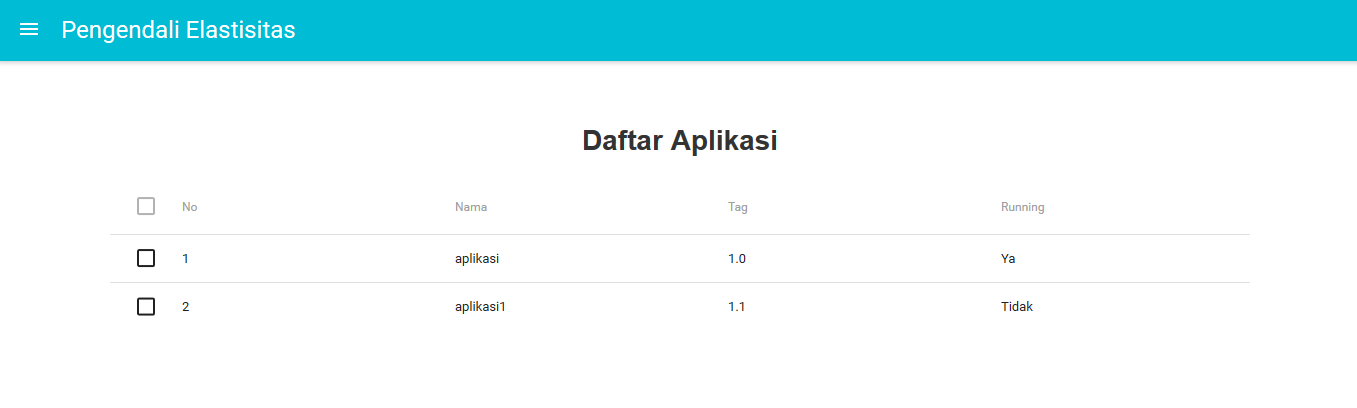
\includegraphics[width=11.2cm,height=3.7cm]{Images/C-4/dasberanda.PNG}
				\caption{Dasbor Daftar Aplikasi}
				\label{ddaftaraplikasi}
			\end{figure}
            
         \subsection{Informasi Aplikasi}
         	\begin{figure}[H]
				\centering
				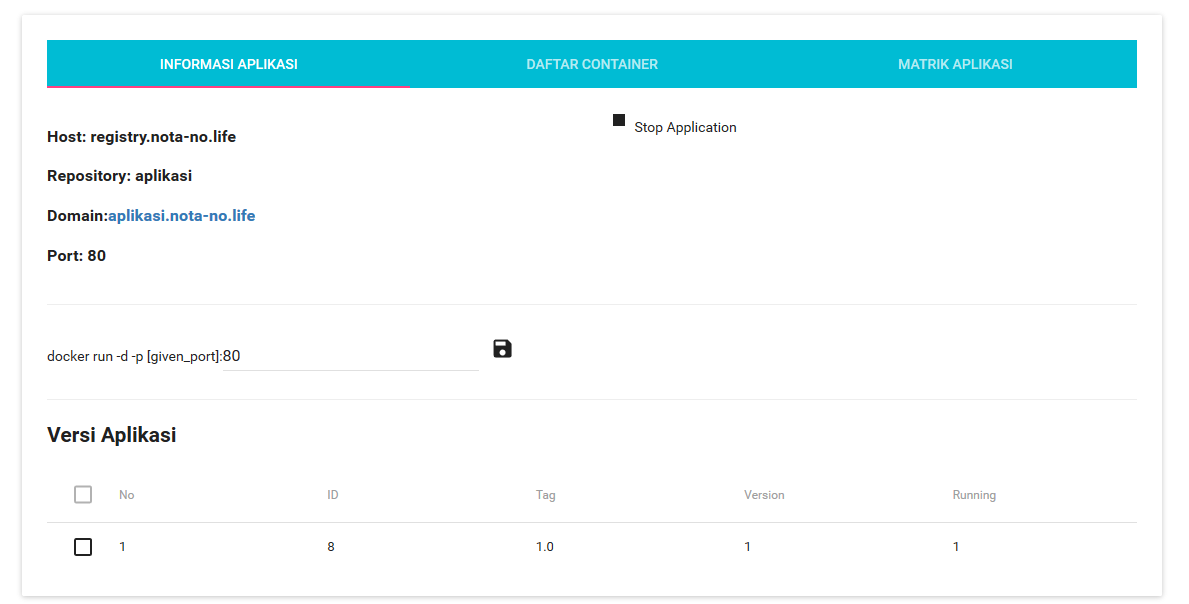
\includegraphics[width=11.2cm,height=9cm]{Images/C-4/dasinformasi.PNG}
				\caption{Dasbor Informasi Aplikasi}
				\label{dinformasiaplikasi}
			\end{figure}
         	Halaman ini menunjukkan infromasi lengkap dari sebuah aplikasi. Pada halaman ini bisa dilihat nama aplikasi, port yang digunakan, domain dari aplikasi, dan versi dari aplikasi. Pada halaman ini, pengguna bisa mengatur port dari aplikasi agar dapat berjalan dengan baik. Dari halaman ini juga aplikasi pertama kali akan dijalankan. Jadi pada halaman ini terdapat kontrol untuk menajalankan dan mematikan aplikasi. Antar muka informasi ditunjukkan pada Gambar \ref{dinformasiaplikasi}.
            
         \subsection{Daftar \textit{Container}}
         	Pada halaman ini, pengguna dapat melihat daftar \textit{container} yang sedang berjalan untuk sebuah aplikasi. Informasi yang diberikan berupa ID dan port dari container. Antar muka halaman daftar \textit{container} ditunjukkan pada Gambar \ref{ddaftarcontainer}.
            \begin{figure}[H]
				\centering
				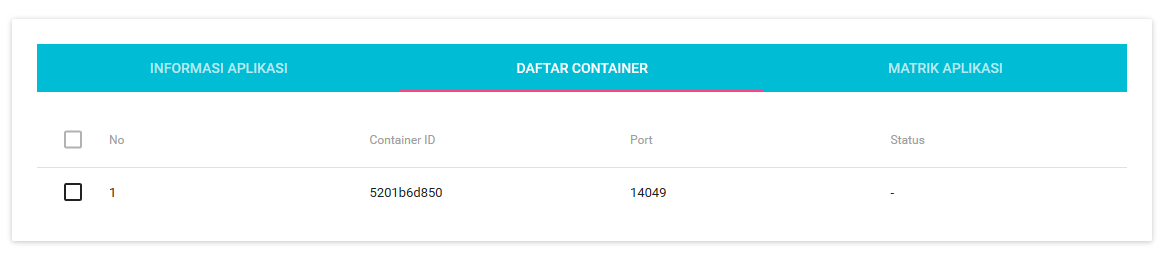
\includegraphics[width=11.2cm,height=3cm]{Images/C-4/dasdafcont.PNG}
				\caption{Dasbor Daftar \textit{Container}}
				\label{ddaftarcontainer}
			\end{figure}
            
         \subsection{Metrik Aplikasi}
         	Halaman metrik aplikasi digunakan untuk memantau keadaan sekarang dari aplikasi. Metrik yang diberikan adalah jumlah \textit{request} pengguna ke aplikasi dan jumlah \textit{container} dari aplikasi. Data akan diperbarui sekitar lima detik sekali. Antar muka metrik aplikasi ditunjukkan pada Gambar \ref{dmatrikaplikasi}.
            \begin{figure}[H]
				\centering
				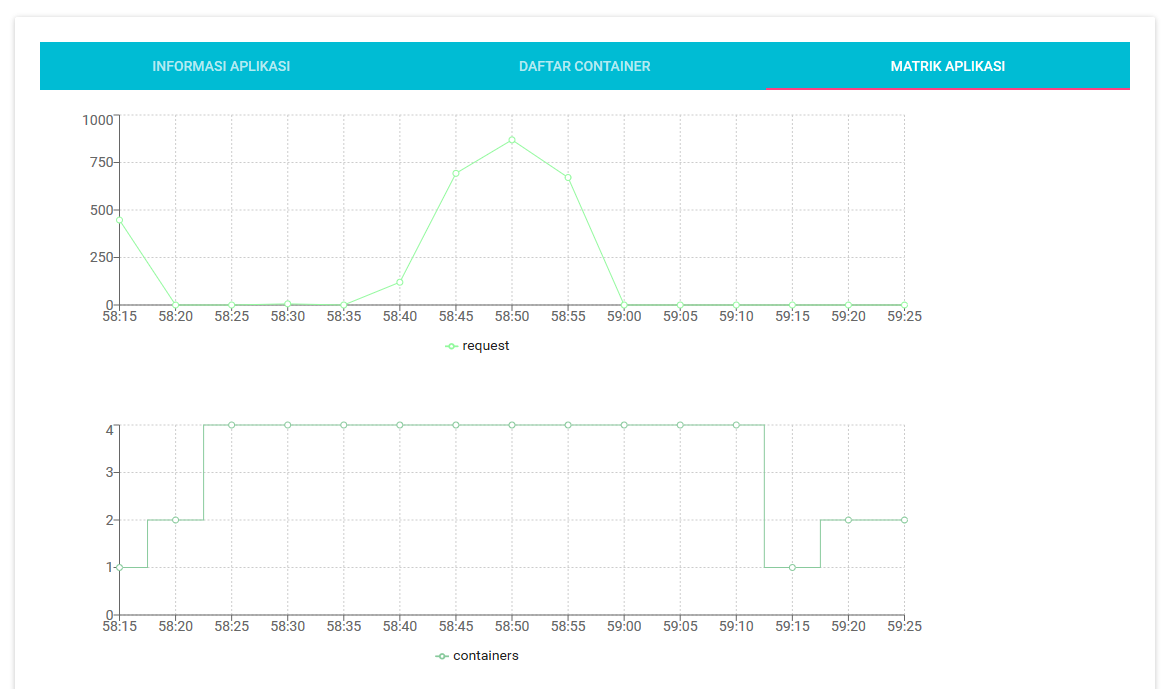
\includegraphics[width=11.2cm,height=7.3cm]{Images/C-4/dasmatrik.PNG}
				\caption{Dasbor Matrik Aplikasi}
				\label{dmatrikaplikasi}
			\end{figure}